\newcommand{\tmp}{TMP36}
\newcommand{\vs}{\texttt{+vs}}
\newcommand{\vout}{\texttt{vout}}
\newcommand{\gnd}{\texttt{gnd}}
\newcommand{\pinV}{\texttt{5v}}
\newcommand{\sensorpin}{\texttt{A0}}
\newcommand{\txtloop}{\texttt{loop}}

\chapter{Misura di Temperature con Arduino}
    Tra le esperienze svolte con Arduino Uno riporto in particolare la misura della variazione della temperatura della mia stanza da letto in seguito all'accensione del riscaldamento in casa.

    \section{L'esperimento}
            L'obiettivo dell'esperienza è quello di valutare qualitativamente l'andamento della temperatura della stanza per fare una stima di quanto velocemente si riscaldi e a quale temperatura tenda asintoticamente.

        \subsection{Preparazione della stanza}\label{ss:ard:preparazione}
            Per massimizzare l'escursione termica ho effettuato la misura durante una sera invernale avendo preventivamente aperto le finestre per abbassare la temperatura della stanza.
            
            Per migliorare la circolazione dell'aria ed evitare un eccessivo gradiente di temperatura---il radiatore caldo si trova in un angolo della stanza mentre i vetri freddi della finestra si trovano dal lato opposto---ho acceso dei ventilatori: uno a soffitto per limitare la raccolta dell'aria calda in alto e un più piccolo ventilatore da tavolo per allontanare l'aria calda dal radiatore e facilitare il riscaldamento dell'aria fredda.
            
            Infine, per isolare il più possbile il sistema, ho chiuso le tende sulla finestra per ridurre la dispersione di calore attraverso il vetro freddo e mantenuto la porta chiusa per non disperdere calore nel resto della casa.

        \subsection{Strumenti utilizzati}
            Gli strumenti utillizzati per la presa dei dati sono:
            \begin{enumerate}[label=$\bullet$]
                \item Una microcontrollore Arduino Uno con un sensore di temperatura \tmp;
                \item Un computer per compilare ed eseguire il codice sulla scheda Arduino e prelevare i dati.
            \end{enumerate}

            Il sensore \tmp\ è un sensore di temperatura a semiconduttore pensato per operare in un range di temperature che va da \SI{-40}{\celsius} a $+\SI{125}{\celsius}$. Esso presenta tre pin: \vs, \vout\ e \gnd. Il primo e l'ultimo servono per l'alimentazione che deve essere compresa tra \SI{2.7}{\volt} e \SI{5.5}{\volt} con una corrente inferiore ai \SI{50}{\micro\ampere}, che garantisce un surriscaldamento per effetto Joule trascurabile. Il secondo pin invece sestituisce una differenza di potenziale rispetto al \gnd\ proporzionale alla temperatura misurata. La sensibilità del sensore fornita dal costruttore è di \SI{\pm 1}{\celsius} e il suo fattore di scala è di \SI{10}{\milli\volt\per\celsius}  \cite{tmp36-datasheet}.

            La scheda Arduino attraverso i pin analogici accetta in input delle differenze di potenziale che vanno da \SI{0}{V} a \SI{5}{V} che vengono convertite in un segnale digitale che assume valori discreti da \num{0} a \num{1023}.

        \subsection{Circuito e codice}\label{ard:codice}
            Il circuito realizzato per l'esperimento è quello rappresentato in \figref{fig:arduino-1}. L'alimentazione al sensore è fornita tramite i pin \pinV\ e \gnd\ mentre il segnale in uscita dal sensore viene letto dal pin \sensorpin\ della scheda.

            \begin{figure}[t]
                \centering
                    \begin{minipage}{0.49\textwidth}
                        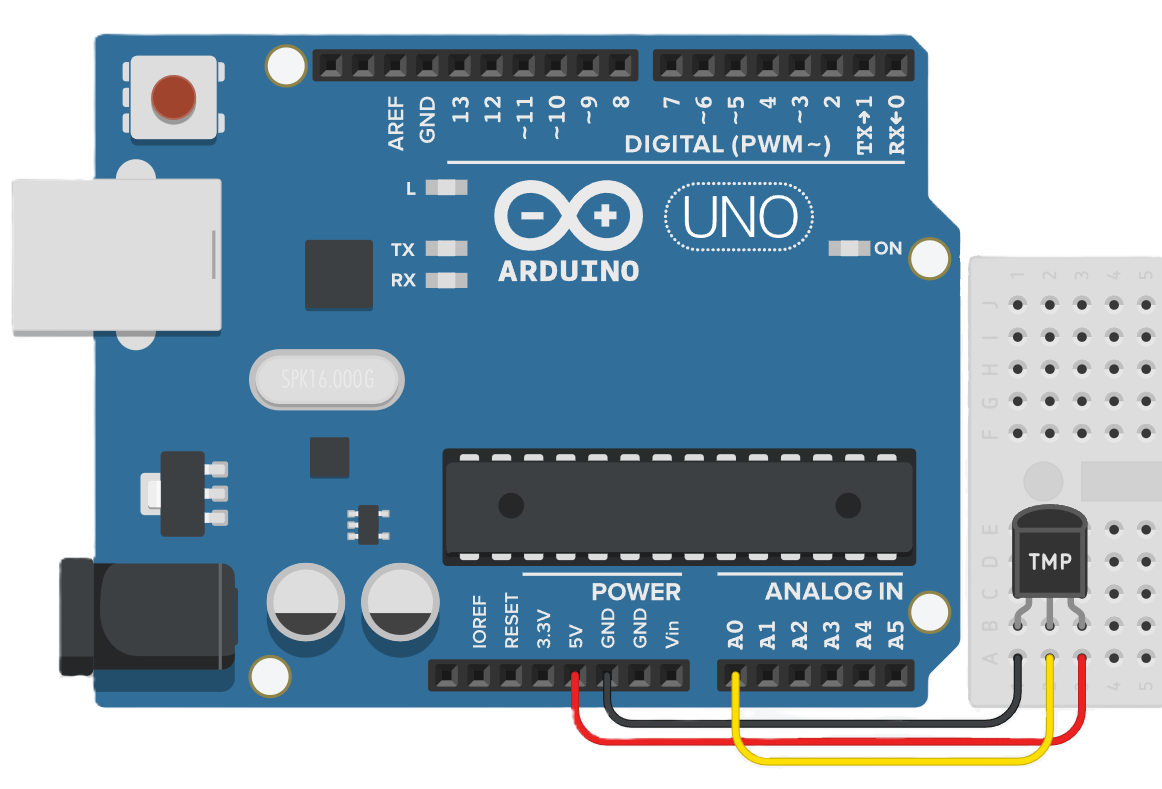
\includegraphics[width = \textwidth]{images/arduino/temp-pic.png}
                    \end{minipage}
                    \hfill
                    \begin{minipage}{0.49\textwidth}
                        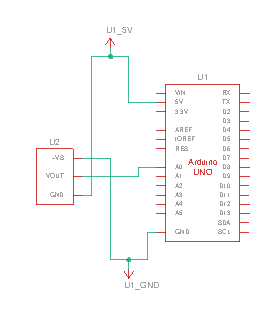
\includegraphics[width = \textwidth]{images/arduino/temp-scheme.pdf}
                    \end{minipage}
                    \caption{A sinistra una rappresentazione digitale del circuito realizzato per l'esperimento. A destra lo schema del circuito. Entrambe le illustrazioni sono state realizzate con Tinkercad\textsuperscript{\textregistered}.}
                    \label{fig:arduino-1}
            \end{figure}

            Per effettuare le misure ho usato il codice riportato di seguito. A intervalli di \SI{30}{\second} la lettura discreta di tensione data dal sensore\footnote{Come detto prima si tratta di un valore tra \num{0} e \num{1023}} e la converte in un numero decimale tra \SI{0}{\volt} e \SI{5}{V} attraverso la formula
            \begin{equation*}
                \frac{\text{\ttfamily (float)analogRead(SENSOR\_PIN)}}{\text{\ttfamily MAX\_READ}} * \text{\ttfamily MAX\_V}
                \mycomma
            \end{equation*}
            essendo $\text{\ttfamily MAX\_READ} = 1023$ e $\text{\ttfamily MAX\_V} = \SI{5}{\volt}$. Sapendo che a una tensione di \SI{0}{\volt} corrisponde una temperatura di \SI{0.5}{\celsius} e a \SI{4.5}{\volt} corrispondono \SI{100}{\celsius}, la conversione della lettura in gradi Celsius è data da
            \begin{equation}
                \bqty{\frac{\text{\ttfamily (float)analogRead(SENSOR\_PIN)}}{\text{\ttfamily MAX\_READ}} * \text{\ttfamily MAX\_V} - \text{\ttfamily A}} * \text{\ttfamily B}
                \mycomma
                \label{eq:ard:temp-conv}
            \end{equation}
            dove $\text{\ttfamily A} = \SI{0.5}{\volt}$ e $\text{\ttfamily B} = \SI{100}{\celsius\per\volt}$ sono i fattori di scala.

            La conversione dei valori discreti in temperatura è eseguita dal codice tra le righe \texttt{23} e \texttt{26} applicando la \eqref{eq:ard:temp-conv}. Vengono eseguite $\text{\ttfamily N} = 20$ misure consecuitive di cui è contestualmente calcolata la media che viene a sua volta stampata a schermo. Infine il codice attende il tempo mancante per raggiungere i \SI{30}{\second} dall'inizio del \txtloop.
            \lstinputlisting[language=C++]{code/arduino-temp.txt}

    \section{Dati}
        Attraverso il codice riportato al punto \S~\ref{ard:codice} ho misurato la temperatura della stanza ogni \SI{30}{s} per circa cinque ore e mezza; in \figref{fig:ard:raw-temp} sono riportati tutti i dati raccolti, avendo convertito il tempo in minuti.

        \begin{figure}
            \centering
            \begin{tikzpicture}
                \begin{axis}[
                    width       = \plotsize,
                    height      = 0.75\plotsize,
                    xlabel      = {Tempo (\unit{\min})},
                    ylabel      = {Temperatura (\unit{\celsius})},
                    xmin        = 0,  xmax = 330, xtick = {0,30,...,330},
                    ymin        = 16, ymax = 28,  ytick = {16,18,...,28},
                    tick align  = outside,
                    colorbar,
                    colormap/hot,
                    point meta  = y
                ]
                    \addplot+ [
                        scatter,
                        only marks,
                        mark        = *,
                        mark size   = 0.5pt,
                        scatter src = y,
                    ] table [
                        x index=0,
                        y index=1,
                        col sep=space
                        ] {code/python/temp_time_conv.dat};
                \end{axis}
            \end{tikzpicture}
            \caption{Andamento della temperatura nel tempo}
            \label{fig:ard:raw-temp}
        \end{figure}%
        \begin{figure}
            \centering
            \begin{tikzpicture}
                \begin{axis}[
                    width       = \plotsize,
                    height      = 0.75\plotsize,
                    xlabel      = {Tempo (\unit{\min})},
                    ylabel      = {Temperatura (\unit{\celsius})},
                    xmin        = 0,  xmax = 330, xtick = {0,30,...,330},
                    ymin        = 18, ymax = 26,  ytick = {18,...,26},
                    extra y ticks       = {24.5},
                    extra y tick labels = {\scriptsize{24.5}},
                    tick align  = outside,
                    legend pos  = south east
                ]
                    \addplot [
                        no marks,
                        draw    = black,
                    ] table [
                        x index = 0,
                        y index = 1,
                        col sep = space
                    ] {code/python/temp_avg.dat};
                    \addplot [
                        domain  = 0 : 330,
                        samples = 1000,
                        color   = red,
                        no marks
                    ] {24.5*(1 - exp(-((x+120)/95)))};
                    \draw[red, dashed] (0, 24.5) -- (330, 24.5);
                    \legend{Dati, Eq.~\eqref{eq:ard:temp-numerica}}
                \end{axis}
            \end{tikzpicture}
            \caption{Temperature mediate in intervalli di \SI{30}{\min}.}
            \label{fig:ard:avg-temp}
        \end{figure}

        \subsection{Prime considerazioni}
            Osservando il grafico si nota una evidente crescita di temperatura che, dopo una crescita regolare, oscilla fino a stabilizzarsi poco sopra i \SI{24}{\celsius}.
            
            I primi punti a temperatura più elevata possono essere dovuti a un precedente contatto con le mani e un riscaldamento del sensore che è poi tornato a temperatura ambiente. L'ampia oscillazione dei dati intorno ai \SI{130}{\min} deve essere dovuta a un movimento del sensore, che ho dovuto spostare di qualche centimetro. È quindi possibile che anche le successive oscillazioni siano dovute alla nuova posizione del sensore in un punto con un flusso d'aria più dinamico.

        \subsection{Breve analisi dei dati}
            Per per visualizzare il macro-andamento della temperatura tamponando il rumore, ho deciso di suddividere le misure in intervalli temporali di \SI{30}{\min} e riportare nel grafico in \figref{fig:ard:avg-temp} la temperatura media per ciascun intervallo.

            Anche in questo caso si notano l'andamento crescente della temperatura e il salto, ma le oscillazioni intorno alla temperatura finale di circa \SI{24}{\celsius} risultano smorzate. Si osserva inoltre che la temperatura si stabilizza intorno a questo valore \SI{150}{\min}---oppure  \SI{2}{\hour}\,\SI{30}{\min}---dopo l'accensione del riscaldamento.
            
            Svolgiamo adesso un fit dei dati di carattere prettamente qualitativo. Dal momento che il radiatore a regime avrà una temperatura $T^*$ fissata e, tenendo conto della dispersione del calore verso l'esterno, è ragionevole assumere che la temperatura della stanza $T\pqty{t}$ tenda asintoticamente a un valore finito $T_\text{f} \leq T^*$ per $t\to+\infty$. Una funzione crescente che ha un comportamento simile è
            \begin{equation}
                T\pqty{t} = T_\text{f}\bqty{1 - \exp\!\pqty{-\frac{t - t_0}{\tau}}}
                \mycomma
                \label{eq:ard:temp-analitica}
            \end{equation}
            per qualche valore di $T_\text{f}$, $t_0$ e $\tau$. Supponiamo arbitrariamente che la temperatura limite\footnote{I dati in \figref{fig:ard:raw-temp} oscillando superano i \SI{25}{\celsius} ma le ultime misure sono tutte comprese tra \SI{24}{\celsius} e \SI{24.5}{\celsius}, motivo per cui assumo quest'ultimo valore come temperatura limite.} sia $T_\text{f} = \SI{24.5}{\celsius}$; per quanto detto prima supponiamo inoltre che il tempo caratteristico\footnote{Dal momento che ``a occhio'' la temperatura di \SI{24.5}{\celsius} viene già raggiunta dopo \SI{150}{\min}, scegliamo il tempo caratteristico come il tempo necessario a raggiungere il \SI{63}{\%}, ovvero \textit{$\pqty{1/e}$-esimo} della temperatura finale.} sia $\tau = \SI{95}{min} \approx$ \SI{63}{\%} di \SI{150}{\min}. Imponendo che sia $T\pqty{0} = \SI{18.63}{\celsius}$ troviamo
            \begin{equation*}
                t_0
                = \tau \log\!\bqty{1-\frac{T\pqty{0}}{T_\text{f}}}
                \approx -\SI{135}{\min}
                \myperiod
            \end{equation*}

            Infine per centrare meglio la funzione rispetto agli intervalli di \SI{30}{\min} sommiamo a $t_0$ un valore di \SI{15}{\min}, pari a metà dell'intervallo di tempo. La funzione finale che si ottiene sostituendo questi valori nella \eqref{eq:ard:temp-analitica} e si trova rappresentata in \figref{fig:ard:avg-temp} è
            \begin{equation}
                T\pqty{t} =  24.5 \bqty{1 - \exp\!\pqty{-\frac{t + 120}{95}}}
                \myperiod
                \label{eq:ard:temp-numerica}
            \end{equation}

    \section{Conclusioni}
        I dati presi possono essere ulteriormente migliorati facendo maggiore attenzione a non toccare gli strumenti o uscendo dalla stanza e assicurandosi che la porta non venga mai aperta.

        Per avere informazioni più dettagliate sulla bontà del fit si potrebbe invece procedere applicando il metodo dei minimi quadrati per determinare i tre parametri $T_\text{f}$, $t_0$ e $\tau$. Per eseguire un fit con due parametri invece che tre, si può migliorare l'accuratezza su $T_\text{f}$ continuando a prendere dati il più a lungo possibile. Questo permetterebbe di fissare la temperatura limite con più sicurezza e di determinare $t_0$ e $\tau$ attraverso la linearizzazione della \eqref{eq:ard:temp-analitica} in
        \begin{equation*}
            \log\!\bqty{1-\frac{T\pqty{t}}{T_\text{f}}} = \frac{t_0}{\tau} - \frac{1}{\tau}t 
            \quad\iff\quad 
            y\pqty{t} = c_1\pqty{t_0,\tau} + c_2\pqty{t_0,\tau}t
            \myperiod
        \end{equation*}

        Si potrebbe inoltre provare a utilizzare funzioni diverse dalla \eqref{eq:ard:temp-analitica} nel fit per provare a modellare quantitativamente le oscillazioni che si verificano in prossimità della temperatura limite, possibilmente dovute a moti convettivi non del tutto smorzati dai ventilatori indicati al punto \S~\ref{ss:ard:preparazione}.
        